\documentclass[11pt, a4paper]{article}

\usepackage{jheppub}

\setlength{\parskip}{1em}
\usepackage{indentfirst}

\usepackage[colorlinks=true, linkcolor=blue, urlcolor=blue, citecolor=blue]{hyperref}
\usepackage{amsmath,amsfonts,amssymb,amsthm,natbib,graphicx,mathtools,mathrsfs}
\usepackage{braket}
\usepackage{enumitem}
\usepackage{hyperref,pgfplots,siunitx}
\usepackage[outdir=./]{epstopdf}
\usepackage{slashed}
\usepackage{caption}


\sisetup{detect-all}
\pgfplotsset{compat=1.18}

\theoremstyle{definition}
\newtheorem{defn}{Definition}[section]
\newtheorem{rmk}[defn]{Remark}
%\newtheorem{note}[defn]{Note}
\newtheorem{notation}[defn]{Notation}

\theoremstyle{plain}
\newtheorem{lemma}[defn]{Lemma}
\newtheorem{prop}[defn]{Proposition}
\newtheorem{thm}[defn]{Theorem}

\begin{document}

\begin{titlepage}
    \centering
    {\huge \bfseries Local Gauge Anomalies and The Standard Model \par}
    \vspace{1cm}
    {\Large \itshape E. Arnold \& K. Okeyre\par}
    \vfill
    {\Large October 2025 \par}
    {\Large Undergraduate Summer Research Project \par}
    {\Large Durham University \par}
\end{titlepage}

\section*{Abstract}
Abstract here
\newpage

\tableofcontents
\newpage

\section{Introduction}

The following report is aimed at undergraduate 
students familiar with lagrangian mechanics, hamiltonian mechanics,
quantum mechanics, and topology. For a guide to the expected prerequisite knowledge see \cite{mathphys1, mathphys2, topnotes}.

[The aim of this report is to offer a gentle 
introduction to quantum field theory, and offer 
insight into one example of where topology shows up 
in theoretical physics.] - CHANGE THIS

Explain structure of report here. 

\section{Quantum States}

One should be familiar with the notion of a quantum wavefunction, such as 
$\psi(x)$, which describes the position of a particle. 
However, in quantum field theory we deal with a more 
abstract concept called a quantum state.

\begin{defn}
Define Hilbert space
\end{defn}

\begin{notation}
We use the Bra-Ket notation for vectors in Hilbert space. A 
vector is written as $| \psi \rangle$ and a covector is 
written as $\langle \phi |$. We define \[ \langle \phi | \psi \rangle := \langle \phi | (| \psi \rangle) \]
Given a vector 
$| \psi \rangle$ the corresponding hermition transpose of 
this vector is $\langle \psi |$, meaning 
$|\psi|^2 = \langle \psi | \psi \rangle$.
\end{notation}

A quantum state is a mathematical entity that embodies all 
the known information of some given quantum system. There 
are two types of quantum states, pure and mixed. We will 
only explain pure quantum states in this section.

A (pure) quantum state is an abstract vector in a complex 
Hilbert space, denoted by $| \psi \rangle $. This Hilbert 
space is called our state space and often has infinite 
dimensions.

Observables of our quantum system correspond to Hermition 
operators on our state space. The eigenvalues of such an 
operator are real and correspond to possible observed 
values. It can be shown that the eigenstates of any 
Hermition operator form a basis for our state space. This 
allows us to relate quantum states to the more familiar 
notion of a quantum wavefunction.

Let $\langle \psi |$ be a quantum state and $\hat{X}$ be the position operator with eigenstates $|x \rangle$. Then $\psi (x) = \langle x | \psi \rangle$. WHY???


\section{The Heisenburg Picture of Quantum Mechanics}

One is usually introduced to quantum mechanics in the 
Schrödinger picture, however, in quantum field theory, 
it is more natural to consider the Heisenburg picture.

In the Schrödinger picture, the quantum states vary with 
time. For example, our quantum state may be represented 
by a wave function $\psi(x,t)$, which evolves in time. 
Conversely,
the operators that act on our state space, such as 
momentum, position, etc, are usually fixed with respect to time. 
The only exception to this is that the Hamiltonian may include 
a potential energy term that varies with time. 

Consider a time dependent quantum state 
$| \psi(t) \rangle$. This state evolves in time 
according the  Schrodinger equation. One can 
represent this via a unitary time-evolution operator 
$U(t,t_0)$ 
as follows;
\[ | \psi(t) \rangle = U(t,t_0) | \psi(t_0) \rangle .\]

In the Schrödinger 
picture, the expectation of a potentially time-dependent hermition operator, $A(t)$, in the 
state $| \psi(t) \rangle$,  can be written as 
\[\langle \hat{A}(t) \rangle = \langle \psi(t) | \hat{A}(t) | \psi(t) \rangle.\]
Choosing some reference time $t_0$ we can rewrite this as
\[\langle \psi(t_0) | \hat{U}\textsuperscript{\textdagger}(t,t_0) \hat{A}  (t) \hat{U}(t,t_0) | \psi(t_0) \rangle.\]
If we define 
\[\hat{A_H}(t) = \hat{U}\textsuperscript{\textdagger}(t,t_0) \hat{A}  (t) \hat{U}(t,t_0) \]
then we have 
\[\langle \hat{A}(t) \rangle = \langle \psi(t_0) | \hat{A_H}(t) | \psi(t_0) \rangle.\]

So we notice that we could have obtained this same 
expectation by considering a constant quantum state 
$| \psi(t_0) \rangle$ and a new operator that evolves with 
time. This is the idea behind the Heisenberg picture of 
quantum mechanics. One interprets the quantum states as 
being fixed in time, and it is the operators that evolve 
in time. 

In the Schrödinger picture, the Schrödinger equation 
governs the time evolution of quantum states. Hence, a 
natural question is, in the Heisenberg picture, how do the 
operators evolve in time?

One can derive the following equation
\[ \frac{d}{dt} \hat{A}_H(t) = \frac{1}{i \hbar} [\hat{A}_H(t), \hat{H}_H(t)] + \left[\frac{d}{dt} \hat{A}_S(t) \right]_H \]
where the subscripts $S$ and $H$ denote whether we are considering the element in the Schrodinger or Heisenberg picture respectively. 

\section{Classical field theory \& Noether's theorem}

\subsection{Classical field theory}
In classical mechanics we consider a countable set of particles
each with finitely many degrees of freedom
and generalised coordinates $q_i(t)$. These generalised coordinates ${\{ q_i(t) \}}_i$ specify
the system's configuration (position in configuration space) and together with the 
generalised conjugate momenta
${\left\{p_i(t) \coloneq \frac{\partial L}{\partial \dot{q}_i} \right\}}_i $ 
define the system's position in phase space.

In classical field theory we generalise this notion of configuration space to a
continuum with infinite degrees of freedom. The scalar field $\phi(t)$ can be seen as
the generalised coordinates of a continuum 
$\left( q_i(t) \xrightarrow{i \rightarrow \vec{x}} \phi(\vec{x}, t) \right)$ and for a system
of continua the set of scalar fields ${\{ \phi_k(\vec{x}, t) \}}_k$
specifies the system's configuration.


Subsequently, we generalise the classical Lagrangian $L(q_i(t), \dot{q}_i(t), t)$ via
\begin{equation}
  L(t) = \int{d^{3}\vec{x}\,\mathcal{L}(\phi_k(\vec{x}, t),\partial_{\mu}\phi_k(\vec{x}, t), \vec{x}, t)}
\end{equation}
where $\mathcal{L}$ is the Lagrangian density. With respect to some path
in configuration space, $\vec{\Phi}(\vec{x}, t)$, the classical action becomes 
\begin{equation}
  S\left[\vec{\Phi}(\vec{x}, t) \right] = \int{dt\,L} 
  = \int{d^4x\,\mathcal{L}(\phi_k(\vec{x}, t),\partial_{\mu}\phi_k(\vec{x}, t), \vec{x}, t)}
\end{equation}
Using Hamilton's principle $\left( \frac{\delta S}{\delta \vec{\Phi} } = 0 \right)$ we obtain
the Euler-Lagrange equations 
\begin{equation}
  \frac{\partial \mathcal{L}}{\partial \phi_k}
  = \partial_\mu \left[ \frac{\partial \mathcal{L}}{\partial(\partial_\mu{\phi_k}) } \right]
\end{equation}
In classical mechanics we define the hamiltonian, $H(p_i(t), q_i(t), t)$, via the
Legendre transform (IS THIS ACTUALLY THE DEFINITION OF H? ASK INAKI)
\begin{equation}
  H = \sum_{i}{p_i(t)\dot{q}_i(t) - L}
\end{equation}
to generalise this to field theory we introduce the momentum field conjugate to 
$\phi_k(\vec{x}, t)$
\begin{equation}
  \pi_k(\vec{x}, t) \coloneq \frac{\partial \mathcal{L} }{\partial \dot{\phi}_k} \\
\end{equation}
\begin{equation}
  p_i(t) \coloneq \frac{\partial L}{\partial \dot{q}_i} \xrightarrow{i \rightarrow \vec{x}}
  \frac{\partial}{\partial \dot{\phi}_k} \left[ \int{d^3\vec{x}\,\mathcal{L}} \right]
  = \int{d^3\vec{x}\,\pi_k(\vec{x}, t)}
\end{equation}
Thus the classical Hamiltonian is generalised to
\begin{equation}
  H(t) = \int{d^3\vec{x}\,\mathcal{H}(\pi_k(\vec{x}, t), \phi_k(\vec{x}, t), \vec{x}, t) }
\end{equation}
\begin{equation}
  \mathcal{H} = \sum_{k}{\pi_k(\vec{x}, t)\dot{\phi}_k(\vec{x}, t) - \mathcal{L}}
\end{equation}
where $\mathcal{H}$ is the Hamiltonian density, and Hamilton's equations become
the Hamiltonian field equations
\begin{equation}
  \dot{\phi}_k = \frac{\partial \mathcal{H}}{\partial \pi_k}
  - \partial_\mu \left[ \frac{\partial \mathcal{H}}{\partial (\partial_\mu \pi_k)} \right],\,
  \dot{\pi}_k = \partial_\mu \left[ \frac{\partial \mathcal{H}}{\partial (\partial_\mu \phi_k)} \right]
  - \frac{\partial \mathcal{H}}{\partial \phi_k}
\end{equation}

[I tried not to use this notation but the rest will be unreadable if I don't, so I hope this
does not contradict following variational deriv notation, also use this notation earlier]
\begin{equation}
  \frac{\delta \mathcal{F}}{\delta g} \coloneq \frac{\partial \mathcal{F}}{\partial g}
  - \partial_\mu \left[ \frac{\partial \mathcal{F}}{\partial (\partial_\mu g)} \right],
\end{equation}

To begin second quantisation we will also require the notion of a field theoretic poisson bracket.
Given two functionals, $F$ and $G$, of the dynamical fields given by 
\begin{equation}
  F = \int{d^3\vec{x}\, \mathcal{F}(\pi_k, \phi_k, \vec{x}, t)},\,
  G = \int{d^3\vec{x}\, \mathcal{G}(\pi_k, \phi_k, \vec{x}, t)}
\end{equation}
We define the poisson bracket
\begin{equation}
  {\{F, G \}}_{f} = \int{d^3\vec{x}\,
  \sum_{k}{\left[ \frac{\delta \mathcal{F}}{\delta \phi_k}\frac{\delta \mathcal{G}}{\delta \pi_k} 
- \frac{\delta \mathcal{G}}{\delta \phi_k}\frac{\delta \mathcal{F}}{\delta \pi_k} \right]}  }
\end{equation}
Note that $K({x}) = \int{d{y}\,[K({y}) \delta(x - y)]}$


\subsection{Noether's first Theorem}
[From here we should somehow state that $\vec{x}$ is a spatial vector and $x$ is a four-vector]

In classical mechanics Noether's first theorem shows the correspondence between global symmetries of 
the lagrangian and conserved quantities called Noether charges. This generalises to global symmetries
of the lagrangian density corresponding to conserved Noether currents in classical field theory.
Consider an infinitesimal field transformation, $\vartheta(\epsilon)$, such that
\begin{equation}
  \phi_k \mapsto \phi_k + \epsilon\vartheta_k(\phi)
\end{equation}
where the generators, $\vartheta_k$, may be a functions of an arbitrary number of fields $\phi_k$ but
are independent of spacetime, and we suppress high order terms in $\epsilon$.
Such a transformation is called a global symmetry if its effect on the Lagrangian density is
\begin{equation}
  \mathcal{L} \mapsto \mathcal{L} + \epsilon\partial_\mu\Lambda^\mu(\phi_k, x)
\end{equation}
This change in the Lagrangian density leaves the Euler-Lagrange equations invariant (add proof L8r).
Noether's theorem for fields states that a transformation $\vartheta(\epsilon)$ is a symmetry
of the lagrangian if and only if 
\begin{equation}
  j^\mu \coloneq
  \sum_{k}{\vartheta_k \frac{\partial \mathcal{L}}{\partial (\partial_\mu \phi_k)}}
  - \Lambda^\mu, \, \partial_\mu j^\mu = 0 
\end{equation}
and the divergence free quantity $j^\mu$ is called the conserved Noether current.
This easily generalises to local symmetries: spacetime dependent generators
$\vartheta_k(\phi, x)$ (add proof L8r).

\section{The Dirac Lagrangian}
[Introduce dirac eqn as relativistic QM,
show U(1) global symm. and that gauging this symm leads to QED lagrangian.
Show we now wish to gauge the axial symm. because of the prev. success but 
at the quantum level there is an anomaly acting as an obstruction to gauging.
From here we use natural units.]

\subsection{Gauging the vector symmetry}

In quantum mechanics the Schrodinger equation is not Lorentz invariant and is thus
incompatible with special relativity. A naive generalisation of the relativistic
dispersion relation using Hamiltonian and momentum operators
for free particles leads to the Klein-Gordon
equation. However, the Klein-Gordon equation is a second order partial differential equation and
subsequently does not uniquely determine time-evolution of the wavefunction.
A more complicated treatment produces the Dirac equation
\begin{equation}
  (i \gamma^\mu\partial_\mu - m)\psi(x) = 0
\end{equation}
Which corresponds to the Lagrangian density
\begin{equation}
  \mathcal{L}_\mathrm{D} = \bar{\psi}(i \gamma^\mu\partial_\mu - m)\psi
\end{equation}
Where the adjoint bispinor is defined as $\bar{\psi} \coloneq \psi^\dagger\gamma^0$.
This Lagrangian admits a global $\mathrm{U}(1)$ symmetry called the vector symmetry
\begin{equation}
  \psi \mapsto e^{i\vartheta}\psi, \quad \bar{\psi} \mapsto \bar{\psi}e^{-i\vartheta} 
\end{equation}
This symmetry corresponds to a conserved vector current via Noether's theorem for fields
[add proof L8R]
\begin{equation}
  j^\mu = \bar{\psi}\gamma^\mu\psi
\end{equation}
We now attempt to `gauge' this symmetry by adding spacetime dependence to the 
parameter
\begin{equation}
  \psi \mapsto e^{i\vartheta(x)}\psi, \quad \bar{\psi} \mapsto \bar{\psi}e^{-i\vartheta(x)}  
\end{equation}
However, the Lagrangian is not invariant under such a transformation so we introduce the
derivative operator which transforms covariantly
\begin{equation}
  D_\mu \coloneq \partial_\mu + ie\Pi_\mu
\end{equation}
\begin{equation}
  D_\mu \psi \mapsto D'_\mu\left[e^{i\vartheta(x)}\psi\right] = e^{i\vartheta(x)}D_\mu\psi
\end{equation}
To satisfy this the gauge field must transform as
\begin{equation}
  \Pi_\mu \mapsto \Pi_\mu -\frac{1}{e}\partial_\mu\vartheta(x)
\end{equation}
Thus we have a modified Lagrangian which admits a local $\mathrm{U}(1)$ gauge symmetry
\begin{equation}
  \mathcal{L} = \bar{\psi}(i\slashed{D} - m)\psi
  = \bar{\psi}(i \gamma^\mu\partial_\mu - m)\psi -e\Pi_\mu j^\mu
\end{equation}
where $\slashed{D} \coloneq \gamma^\mu D_\mu$ is the Dirac operator.
This is strikingly similar to the electromagnetic Lagrangian density which
also has a $\mathrm{U}(1)$ gauge symmetry
\begin{equation}
  \mathcal{L}_\mathrm{EM} = -\frac{1}{4}F_{\mu\nu}F^{\mu\nu} -A_\mu J^\mu
\end{equation}
where $A_\mu$, $J^\mu$, and $F^{\mu\nu}$ are the electromagnetic four-potential, four-current,
and field tensor respectively. Thus we identify $\Pi_\mu = A_\mu$ and $ej^\mu = J^\mu$
and arrive at the Lagrangian for quantum electrodynamics.
\begin{equation}
  \mathcal{L}_\mathrm{QED} = -\frac{1}{4}F_{\mu\nu}F^{\mu\nu} -eA_\mu j^\mu
    + \bar{\psi}(i \gamma^\mu\partial_\mu - m)\psi
\end{equation}

[Speak about how QED is an incredibly successful theory of photon-electron interactions]


\subsection{The Axial symmetry}

However, this is not the end of the story. The massless Dirac Lagrangian admits
another symmetry better seen in the Weyl basis.
\begin{equation}
  \psi =
  \begin{pmatrix} \psi_\mathrm{L} \\ \psi_\mathrm{R} \end{pmatrix}, \quad
  \gamma^{\mu}\partial_\mu =
  \begin{pmatrix}0 & \sigma^\mu\partial_\mu \\ \bar{\sigma}^{\mu}\partial_\mu & 0 \end{pmatrix}
\end{equation}
Thus the Dirac Lagrangian can be seen as the interaction between two Weyl fermions
of opposite chirality
\begin{equation}
  \mathcal{L}_\mathrm{D} = \psi_\mathrm{L}^{\dagger}(i\sigma^\mu\partial_\mu)\psi_\mathrm{L} +
  \psi_\mathrm{R}^{\dagger}(i\bar{\sigma}^\mu\partial_\mu)\psi_\mathrm{R}
  - m(\psi_\mathrm{L}^{\dagger}\psi_\mathrm{R} + \psi_\mathrm{R}^{\dagger}\psi_\mathrm{L})
\end{equation}
In the massless case the Lagrangian gains a global $\mathrm{U}(1)$ symmetry
known as the axial symmetry
\begin{equation}
  \psi_\mathrm{L} \mapsto e^{i\vartheta}\psi_\mathrm{L}, \quad
  \psi_\mathrm{R} \mapsto e^{-i\vartheta}\psi_\mathrm{R}
\end{equation}
which is equivalent to 
\begin{equation}
  \psi \mapsto e^{i\vartheta\gamma^5}\psi
\end{equation}
and a Noether current
\begin{equation}
  j^\mu_5 = \bar{\psi}\gamma^\mu\gamma^5\psi, \quad \partial_\mu j^\mu_5 = 2im\bar{\psi}\gamma^5\psi
\end{equation}
We now proceed as before, gauging the axial symmetry by promoting $\partial_\mu$
to a covariant derivative as in (5.6) and determining the required gauge transformation
\begin{equation}
  {\mathcal{L}_{D}|}_{m=0} = \bar{\psi}(i\gamma^\mu \partial_\mu)\psi
  - q\bar{\psi}\gamma^\mu\Pi_\mu\psi
\end{equation}
\begin{equation}
  \Pi_\mu \mapsto e^{i\vartheta\gamma^5}\Pi_\mu e^{-i\vartheta\gamma^5} 
  - \frac{1}{q}\partial_\mu\vartheta\gamma^5
\end{equation}
Now we must add a kinetic term to the Lagrangian to determine the dynamics 
of the matrix-valued gauge field. Such a term must be gauge-invariant to preserve
the $\mathrm{U}(1)$ symmetry. We find a Lagrangian analogous to the Maxwell Lagrangian
\begin{equation}
  \mathcal{L}_\Pi = - \frac{1}{4}\mathrm{Tr}(\Gamma_{\mu\nu}\Gamma^{\mu\nu})
\end{equation}
with field strength
\begin{equation}
  \Gamma_{\mu\nu} = \partial_\mu\Pi_\nu - \partial_\nu\Pi_\mu +q[\Pi_\mu, \Pi_\nu]
\end{equation}
has the required gauge-invariance and is Lorentz invariant.
Thus we have a theory describing the coupling
of massless dirac fermions to a mysterious gauge field
\begin{equation}
  \mathcal{L} =  - \frac{1}{4}\mathrm{Tr}(\Gamma_{\mu\nu}\Gamma^{\mu\nu}) 
  - q\bar{\psi}\gamma^\mu\Pi_\mu\psi
  + \bar{\psi}(i\gamma^\mu \partial_\mu)\psi
\end{equation}


\section{Quantum Field Theory}

So far we have studied relativistic quantum mechanics, making use of classical
fields to describe the dynamics of quantum states. However, such a quantum theory is
inconsistent subsequently predicting negative energy states which require 
peculiar interpretations to reconcile (Dirac's hole theory). To proceed to a
quantum theory of particle interactions we must promote the dynamical fields
to field operators; second quantisation. We shall see how this shift to
a quantised field theory affects our calculation of expectation values and probabilities.


\subsection{Second Quantisation}
In classical mechanics, the canonical transformations are exactly those which preserve the symplectic 
structure; invariance of poisson brackets of the dynamical variables ($p_i, q_i$) characterises
transformations which leave Hamilton's equations unchanged.
A system's position in phase space specifies its classical state.

However, in quantum mechanics all properties of a system are included in a quantum state, $\ket{\psi}$, 
inside of a Hilbert space upon which operators corresponding to observables act.
Dirac's famous canonical quantisation
rule (${\{A, B \} \rightarrow \frac{1}{i\hbar}[\hat{A}, \hat{B}]}$) allows us quantise 
the canonical structure of classical mechanics (although Groenewold's theorem shows us 
that such a rule cannot hold for all functions of the dynamical variables). 
To obtain a quantised field theory we consider the field theoretic poisson brackets
\begin{equation}
  {\{ \phi_n(z), \phi_m(w) \}}_f = 0 = {\{ \pi_n(z), \pi_m(w) \}}_f
\end{equation}
\begin{equation}
  {\{\phi_n(z), \pi_m(w) \}}_f = \delta_{nm}\delta^{(3)}(\vec{z} - \vec{w})
\end{equation}
Which are quantised to the canonical commutation relations for the dynamical
field operators acting on a Fock space
\begin{equation}
  {[\hat{\phi}_n(z), \hat{\phi}_m(w) ]} = 0
  = {[\hat{\pi}_n(z), \hat{\pi}_m(w) ]}
\end{equation}
\begin{equation}
  {[ \hat{\phi}_n(z), \hat{\pi}_m(w) ]}
  = i\hbar\delta_{nm}\delta^{(3)}(\vec{z} - \vec{w})
\end{equation}
However, just like Dirac's rule this procedure does not always produce a consistent quantum
theory and in the case of quantising the Dirac Lagrangian we require the analogous anti-commutation
relations because of the spin-statistics theorem.
In principle, commutation relations are axioms of any quantum theory
chosen to reproduce experimental observations.


\subsection{Fock Space}
After second quantisation in general we obtain an expression for the Hamiltonian operator
in terms of various creation and annihilation operators (e.g. $a^{r\dagger}_{\vec{p}_1},
b^{s\dagger}_{\vec{p}_2}, \dots$ and $a^{r}_{\vec{p}_1}, b^{s}_{\vec{p}_2}, \dots$ 
respectively). Subsequently we define the vacuum state to be annihilated by
all particle annihilation operators
\begin{equation}
  {a^{r}_{\vec{p}_1}}\!\!\ket{0} = b^{r}_{\vec{p}_1}\!\!\ket{0} = \dotsi = 0
\end{equation}
The indistinguishable $n$-particle state is given by 
\begin{equation}
  a^{r_1\dagger}_{\vec{p}_1}a^{r_2\dagger}_{\vec{p}_2}\dotsi
  a^{r_n\dagger}_{\vec{p}_n}\!\!\ket{0} =
  \ket{r_1, \vec{p}_1; r_2, \vec{p}_2; \dots; r_n, \vec{p}_n} \in H^{\otimes n}
\end{equation}
\begin{equation}
  H^{\otimes n} \coloneq \bigotimes_{k=1}^{n}{H}
\end{equation}
Where $H^{\otimes n}$ is the $n$-particle Hilbert space ($H^0 = \mathbb{C}$ 
corresponds to the vacuum),
and an arbitrary quantum state is an element of the Fock space
\begin{equation}
  F(H) \coloneq \bigoplus_{n=0}^{\infty}{H^{\otimes n}}
\end{equation}
Thus the probability amplitude of a state transitioning from one particle to 
another is
\begin{equation}
  \braket{r_2, \vec{p}_2|r_1, \vec{p}_1} =
  \Braket{0|a^{r_2}_{\vec{p}_2}a^{r_1\dagger}_{\vec{p}_1}|0} \coloneq 
  \Braket{a^{r_2}_{\vec{p}_2}a^{r_1\dagger}_{\vec{p}_1}}
\end{equation}
which generalises to transitions between arbitrary quantum states.
Hence in quantum field theory the study of probabilities is
characterised by vacuum expectation values of operators and their compositions.

\newpage

\section{Path Integral Formulation of Quantum Mechanics}

\subsection{The Propagator}
In quantum mechanics, the propagator is the probability 
amplitude of observing a position $x_n$ at time $t_n$, given 
the particle is at postion $x_1$ at time $t_1$. This can be 
written as the scalar product of the two quantum states,
\begin{equation} 
K(x',t';x,t) := \langle x't'|xt \rangle .
\label{propagator}
\end{equation}

We can rewrite this propagator as an integral over all 
possible paths the particle can take. We call this the 
Feynman path integral.

First, we discretise the time between $t_n$ and $t$ as
\[ t_{n+1} := t'>t_{n}>t_{n-1}>...>t_2>t_1>t =: t_0 ,\]
giving $n+1$ equal peices $\Delta t = t_j-t_{j-1}$ for 
$1 \leq j \leq n+1$.

Since position eigenstates are complete, we have
\begin{equation} 
\int dx_j |x_jt_j \rangle \langle x_jt_j | = \mathbb{I},
\end{equation}
meaning we can rewite \eqref{propagator} as
\begin{align} 
K(x',t';x,t) =
\int dx_{n}dx_{n-1}...dx_1 
&\langle x_{n+1}t_{n+1}|x_{n}t_{n} \rangle
\langle x_{n}t_{n}|x_{n-1}t_{n-1} \rangle
... \notag \\
&...\langle x_{2}t_{2}|x_{1}t_{1} \rangle
\langle x_{1}t_{1}|x_{0}t_{0} \rangle .
\label{pathint}
\end{align}

This can be thought of as integrating over all possible 
paths, as depicted in Figure \ref{figpaths}.

\begin{figure}[h!]
\centering
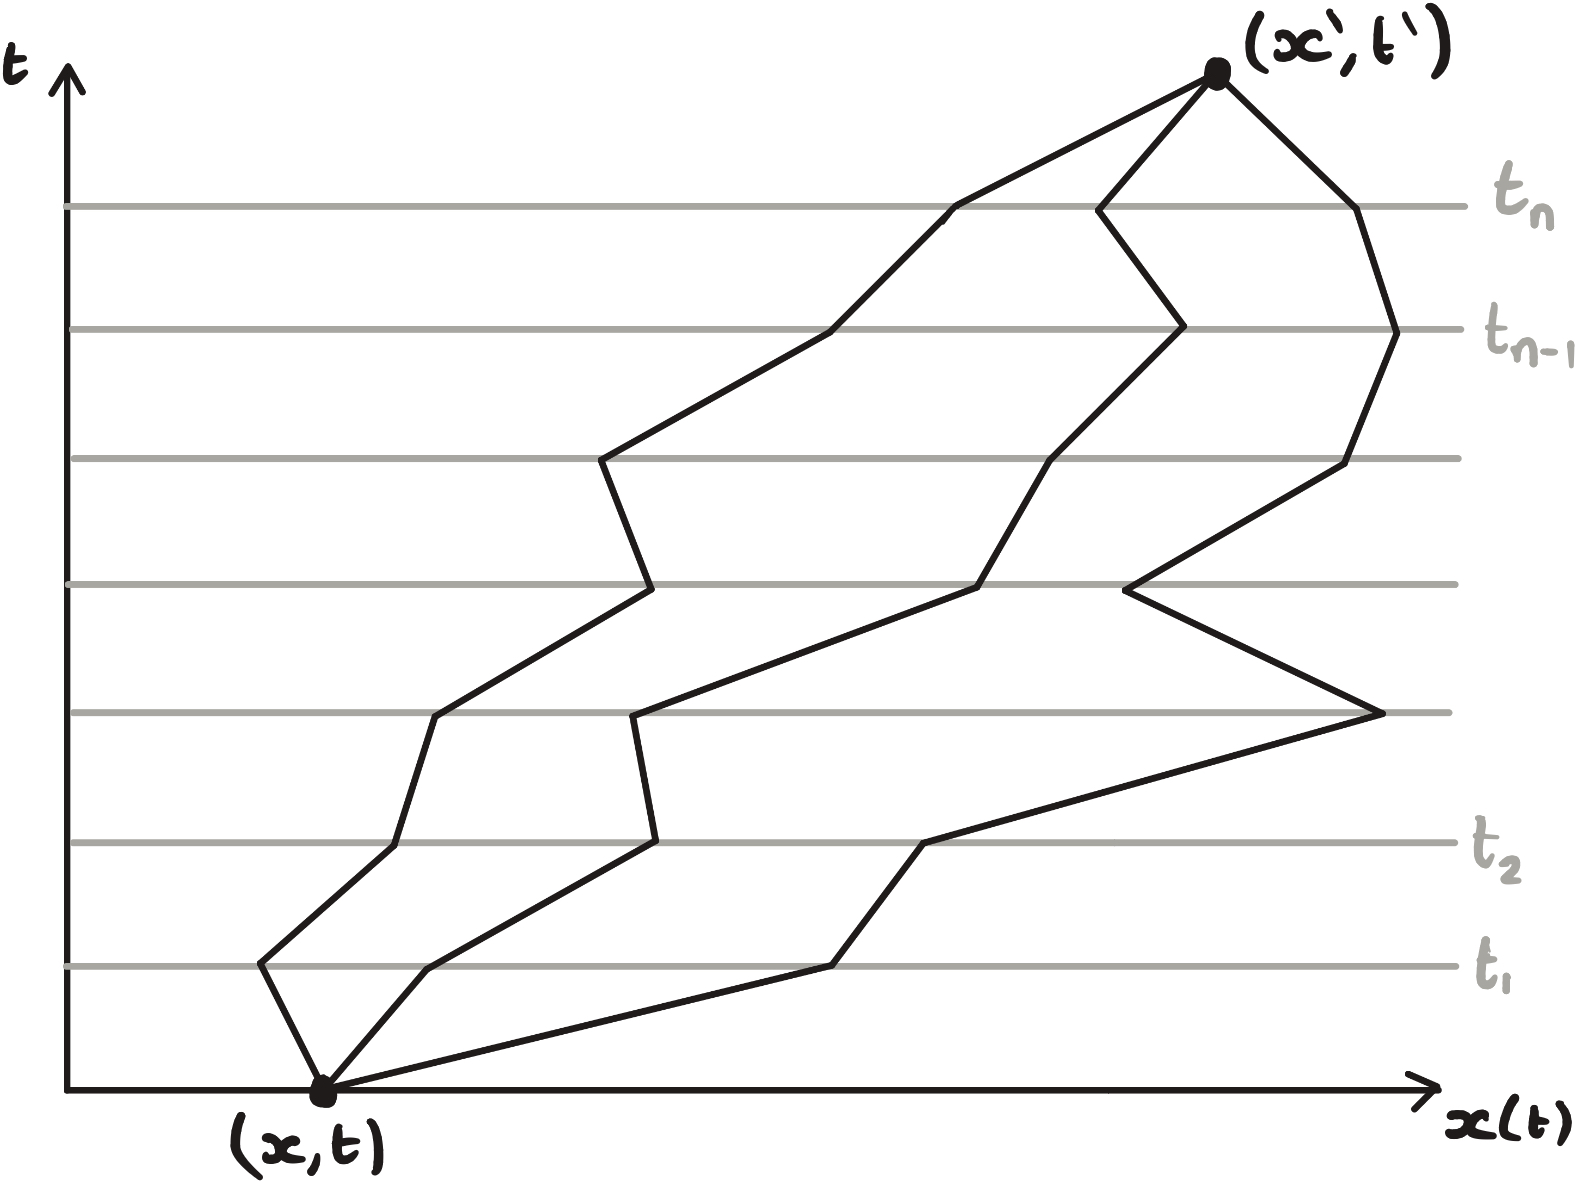
\includegraphics[width=0.4\textwidth]{paths.jpeg}
\captionsetup{width=0.6\textwidth}
\caption{Three possible paths from $(x,t)$ to $(x',t')$ with discretised time interval.}
\label{figpaths}
\end{figure}

Dirac and Feynman cite(dirac, feynman) showed that for 
small $\Delta t$ the path of a particle is determined 
by the classical action, S, via the following,
\begin{equation}
\langle x_jt_j | x_{j-1}t_{j-1} \rangle
=
A \ exp \left\{\frac{i}{h}S(j,j-1)\right\}
\label{pathofsmall}
\end{equation}
where $A$ is a normalisation constant.

$S$ is the classical action determined by the time integral 
of the Lagrangian. As we let $\Delta t \longrightarrow 0$ we 
can approximate the path as a straight line, allowing us to 
calculate the Lagrangian, and hence the action.
\begin{align}
    S(j,j-1) &= \int^{t_j}_{t_{j-1}} dt L_{classical}(x, \dot{x}) \notag \\
    &= \int^{t_j}_{t_{j-1}} dt \left[ \frac{\mu \dot{x}^2}{2} - V(x) \right] \notag \\
    &= \Delta t \left[ \frac{\mu}{2} \left(\frac{x_j - x_{j-1}}{\Delta t} \right)^2 
    - V \left(\frac{x_j + x_{j-1}}{2} \right) \right] \\
    &are these second and third lines neccessary? \notag
\end{align}
Note that one can show $A = \left(\frac{\mu}{2 \pi \hbar i \Delta t} \right)^{\frac{1}{2}}$.

Subbing \eqref{pathofsmall} into \eqref{pathint} and 
taking the limit as $N \longrightarrow \infty$ and 
$\Delta t \longrightarrow 0$ gives
\begin{align}
K(x',t';x,t) &= \lim_{\substack{n \to \infty \\ \Delta t \to 0}} \left[ \left(\frac{\mu}{2 \pi \hbar i \Delta t} \right)^{\frac{n+1}{2}}
\int dx_{n}dx_{n-1}...dx_1 \prod_{j=1}^{n}exp \left\{\frac{i}{h}S(j,j-1)\right\} \right] \notag\\
&= \lim_{\substack{n \to \infty \\ \Delta t \to 0}} \left[ \left(\frac{\mu}{2 \pi \hbar i \Delta t} \right)^{\frac{n+1}{2}}
\int dx_{n}dx_{n-1}...dx_1 \ exp \left\{ \frac{i}{h} \sum_{j=1}^n S(j,j-1)\right\} \right] \notag\\
&= \lim_{\substack{n \to \infty \\ \Delta t \to 0}} \left[ \left(\frac{\mu}{2 \pi \hbar i \Delta t} \right)^{\frac{n+1}{2}}
\int dx_{n}dx_{n-1}...dx_1 \ exp \left\{ \frac{i}{h} \sum_{j=1}^n \int_{j-1}^{j} L_{clasical}(x, \dot{x})\right\} \right] \notag\\
&= \lim_{\substack{n \to \infty \\ \Delta t \to 0}} \left(\frac{\mu}{2 \pi \hbar i \Delta t} \right)^{\frac{n+1}{2}}
\int dx_{n}dx_{n-1}...dx_1 \ exp \left\{ \frac{i}{h} \sum_{j=1}^n \int_{t_0}^{n+1} L_{clasical}(x, \dot{x})\right\}
\\need to fix this equation
\end{align}

\begin{prop}
The Feynman path integral is equivalent to Schrödinger's theory.
\end{prop}

\subsection{The Partition Function}
We consider a system that evolves from a vacuum state at $t \to -\infty$ back to 
a vacuum state at $t \to \infty$, in the 
presence of a source. A vacuum state is a groundstate with zero quantum number (what?). 

The source is introduced 
in the Lagrangian by 
\begin{equation}
L \to L + \hbar J(t)x(t),
\end{equation}
where $J(t)$ is the source and $x(t)$ is the path.

We define the partition function as the transition amplitude in the presence of this source,
\begin{equation}
Z[J]:= \langle 0,-\infty ; 0, \infty \rangle ^J,
\end{equation}
which one can prove is equivalent to 
\begin{equation}
Z[J]= \int d[x(t)] exp\left\{\frac{i}{\hbar}\int^{\infty}_{-\infty}dt (L + \hbar J(t) x(t) + \frac{1}{2} i \epsilon x^2) \right\}.
\end{equation}
what is epsilon?



\subsection{Time Ordered Products}
AKA greens functions
\subsection{Functional Derivatives of the Partition Function}
This is why the partition function is aolso called generating functional

\section{Generalising the Path Integral to Quantum Field Theory}
In the same way we generalised classical mechanics to 
classical field theory in section ---, we can generalise 
quantum mechanics to quantum field theory. That is, instead 
of considering trajectories of a particle x(t), we

maybe talk about why deriving the PI approach to QFT is difficult

talk about how generating functional generalises and how time ordered products generalise to operators I think?

\section{Anomalies in QFT}

\subsection{Symmetries \& Slavnov-Taylor identities}
We now extend our investigation of symmetries from classical fields to a
quantised theory. Suppose the classical action admits a local symmetry
such that the path integral measure is invariant
\begin{equation}
  \phi_\mu \mapsto \phi_\mu + \epsilon\vartheta_\mu(\phi, x)
\end{equation}
\begin{equation}
  \mathcal{D}\phi \mapsto
  \mathcal{D}\phi\,\det\!{\left(\frac{\partial \phi'_{\mu}(x)}{\partial \phi_\nu(y)}\right)}
  = \mathcal{D}\phi
\end{equation}
where $K_{\mu\nu} = \frac{\partial \phi'_{\mu}(x)}{\partial \phi_\nu(y)}$ is the 
transformation Jacobian. Thus the partition function is invariant
and for a source $J^\mu$ corresponding to $\phi_\mu$ we can write [ADD PROOF L8R]
\begin{equation}
  \int{d^4x\,J^\mu(x)\!\braket{\vartheta_\mu(\phi, x)}}_J = 0
\end{equation}
The quantum action is $W[J] = -i\ln{Z[J]}$, and 
we define the effective quantum action as the Legendre transform
\begin{equation}
  \Gamma[\varphi] = W[J] - \int{d^4x\,J^\mu(x)\varphi_\mu(x)} \quad; 
  \quad \varphi_\mu \coloneq \braket{\phi_\mu}_J
\end{equation}
Taking the functional derivative we obtain
\begin{equation}
  J^\mu(x) = - \frac{\delta \Gamma[\varphi]}{\delta \varphi_\mu(x)}
\end{equation}
Subsequently using (9.3) and the definition of a functional derivative 
\begin{equation}
  \delta\Gamma[\varphi_\mu;\braket{\vartheta_\mu(\phi, x)}_J] = 0
\end{equation}
Thus the effective quantum action is invariant under the transformations
\begin{equation}
  \varphi_\mu \mapsto \varphi_\mu + \epsilon\!\braket{\vartheta_\mu(\phi, x)}_J 
\end{equation}
such a relation is called a Slavnov-Taylor identity.
If the transformation is a linear symmetry such that
\begin{equation}
  \vartheta_\mu = \Theta_\mu[\phi, x] = \alpha_\mu(x) +
  \int{d^4y\,\beta^\nu_\mu(x, y)\phi_\nu(y) }
\end{equation}
the transformation Jacobian becomes field independent
\begin{equation}
  K_{\mu\nu} = \frac{\delta}{\delta\phi_\nu(y)}[\phi_\mu +\epsilon\Theta_\mu(\phi, x)]
  = \delta_{\mu\nu}\delta^{(4)}(x - y) + \epsilon\beta^\nu_\mu(x, y)
\end{equation}
so the normalised correlators are invariant. Moreover, we have
$\braket{\Theta_\mu(\phi, x)}_J = \Theta_\mu(\varphi, x)$ which implies
the effective quantum action is invariant under the same transformation as the 
classical action, namely,
\begin{equation}
  \varphi_\mu \mapsto \varphi_\mu + \epsilon\Theta_\mu(\varphi, x)
\end{equation}
is a symmetry. In this case the quantum theory inherits the classical symmetry
and it is impossible to violate the symmetry via quantum effects granted
a regularisation procedure which respects the effective quantum
action's symmetry is employed. However, it is possible that no regularisation
can preserve a classical symmetry, such a symmetry is called an anomaly and
is characterised using the Atiyah–Singer index theorem.
Returning to the Dirac Lagrangian, the vector and axial symmetries are linear
in the fields but without identifying symmetry preserving regularisations 
their accession to a quantum theory is undetermined.

\subsection{The Path Integral measure}

To further investigate the effect of transformations on the partition function
we must introduce a more precise notion a path integral for fermionic fields.

We decompose the Dirac spinor and its adjoint using an orthonormal basis $\{ \phi_n(x) \}$ of
the Dirac operator's eigenfunctions and the independent Grassmann variables 
$\theta_n$ and $\bar{\xi}_m$
\begin{equation}
  \psi = \sum_n{\theta_n\phi_n(x)} = \sum_n{\theta_n\!\braket{x|n}}
\end{equation}
\begin{equation}
  \bar{\psi} = \sum_m{\bar{\xi}_m\phi^{\dagger}_m(x)} = \sum_m{\bar{\xi}_m\!\braket{m|x}}
  \end{equation}
Hence the path integral measure can be seen as a transformation of a Grassmann measure
under a change of variables
\begin{equation}
  \theta \mapsto A\theta = \theta_n\braket{x|n},\quad
  \bar{\xi} \mapsto \bar{\xi}B^{\dagger} = \bar{\xi}_m\braket{m|x}
\end{equation}
\begin{equation}
  \prod_n{d\theta_n}\prod_m{d\bar{\xi}_m} \mapsto \mathcal{D}\psi\mathcal{D}\bar{\psi}
  = {(\det{A}\det{B^\dagger})}^{-1}\prod_n{d\theta_n}\prod_m{d\bar{\xi}_m}
  = \prod_n{d\theta_n d\bar{\xi}_n} 
\end{equation}
Under the infinitesimal vector transformation the Dirac spinor becomes
\begin{equation}
  \psi' = \sum_n{\theta_n'\phi_n(x)} ;\quad \theta_n' = e^{i\vartheta(x)}\theta_n
\end{equation}
and similarly for the adjoint spinor. Thus the path integral measure transforms as
\begin{equation}
  \mathcal{D}\psi\mathcal{D}\bar{\psi} \mapsto
  {\left[\det\left(e^{i\vartheta(x)\mathbb{I}}\right)\right]}^{-2} \mathcal{D}\psi\mathcal{D}\bar{\psi}
\end{equation}
and using the identity
\begin{equation}
  \det\left( e^{A}\right) = e^{\mathrm{Tr}(A)}
\end{equation}
we see the measure changes by a pure phase only; the vector symmetry is retained
by the quantum theory and the correlators are gauge invariant.
However, this is not the case for the axial transformation
where the Grassmann variables transform as
\begin{equation}
  \theta_n' = \sum_m{C_{nm} \theta_m} ,\quad \bar{\xi}_n' = \sum_m{C_{nm} \bar{\xi}_m}
\end{equation}
\begin{equation}
  C_{nm} = \delta_{nm} +i\int{dx\, \vartheta(x)\phi_{n}^{\dagger}(x)\gamma^5\phi_m(x)}
\end{equation}
and the path integral measure changes by the Jacobian
\begin{equation}
  J[\vartheta] = {(\det{C})}^{-2} = \exp\left[-2 \mathrm{Tr}(\ln{C}) \right]
\end{equation}
Expanding the matrix logarithm to first order in the infinitesimal parameter
\begin{equation}
  \ln{(\mathbb{I} + \epsilon A)} = \epsilon A
\end{equation}
we obtain
\begin{equation}
  J[\vartheta] = \exp{\left[-2\mathrm{Tr}\left(i
  \int{dx\,  \vartheta(x)\phi_{n}^{\dagger}(x)\gamma^5\phi_m(x)} \right) \right]}
\end{equation}
\begin{equation}
  J[\vartheta] = \exp{\left[ -2i
  \int{dx\,\vartheta(x) \sum_n{\phi_{n}^{\dagger}(x)\gamma^5\phi_n(x)}} \right]}
\end{equation}
However the sum appearing in the Jacobian is clearly divergent (by orthonormality)
and requires the introduction of a regulator or ultraviolet cut-off to obtain a
non-singular Jacobian.But there is a much more elegant approach available involving 
the Atiyah–Singer index theorem.

\subsection{Atiyah–Singer index Theorem}

[Here our task is to show (maybe just state) what the Jacobians of the vector and axial 
symms are and show that we can always write a relationship between the
index of a differential operator and the divergence of a current. By using
the AST we should find the analytical index and topological index of
a differential operator coincide. My guess is the topological index should
be the same using any `sensible' regularisation thus the anomaly should
persist.]

Given an eigenfunction of the Dirac operator, $\phi_n$, with an eigenvalue $\lambda_n \neq 0$ 
,$\gamma^5\phi_n$ is also an eigenfunction
\begin{equation}
  \slashed{D}(\gamma^5\phi_n) = -\gamma^5\slashed{D}(\phi_n) = -\lambda_n\gamma^5\phi_n
\end{equation}
and the two are orthogonal as they have different eigenvalues.
However, when the eigenvalue is zero $\phi_n$ and $\gamma^5\phi_n$ correspond to $\lambda_n = 0$
and are called zero modes of $\slashed{D}$. We also have that $\gamma^5$ is 
hermitian thus by the spectral theorem there is a basis that diagonalises $\gamma^5$
and spans $\mathrm{Ker}(\slashed{D})$. The eigenvalues of $\gamma^5$ are $\pm 1$
(because ${(\gamma^5)}^2 = I_4$) and we use the projection
operators $P_\pm = \frac{1}{2}(I_4 \pm \gamma^5)$ to decompose
spinors into their positive and negative eigenvalue (positive and negative chirality respectively)
components. Ignoring the infinitesimal parameter for now, only the zero modes contribute
to the integral in the Jacobian because of orthonormality and we have
\begin{equation}
  \int{dx\, \sum_n{\phi^\dagger_n\gamma^5\phi_n}}
  = \sum_n{\int{dx\,\phi^{0\dagger}_{n+}\phi^0_{n+}}}
  -\sum_n{\int{dx\,\phi^{0\dagger}_{n-}\phi^0_{n-}}} = n_+ - n_-
\end{equation}
where $n_\pm$ are the number of positive and negative chirality zero modes $\phi^0_{n\pm}$
respectively. This is precisely the analytical index of the Dirac operator 
projected onto the positive chirality subspace
\begin{equation}
  \mathrm{index}(\slashed{D}|_{\{+\}}) = n_+ - n_- 
\end{equation}
\begin{equation}
  \slashed{D}P_{\pm} = \slashed{D}|_{\{\pm\}} 
\end{equation}
By the Atiyah–Singer index theorem this coincides with the Dirac operator's 
topological index
\begin{equation}
  \mathrm{index}(\slashed{D}|_{\{+\}}) = - \frac{e^2}{32\pi^2}\int{dx\,
  \varepsilon^{\mu\nu\rho\sigma}F_{\mu\nu}F_{\rho\sigma}}
\end{equation}
one can also show this is also the divergence of the axial current using Feynman diagrams.
Thus the axial symmetry is anomalous and the Jacobian is
\begin{equation}
  J[\vartheta] = \exp{\left[-\int{dx\,\vartheta(x)\mathcal{A}[A_\mu]}\right]}
\end{equation}
where $\mathcal{A}$ is the axial anomaly given by
\begin{equation}
  \partial_\mu j^\mu_5 = \mathcal{A}[A_\mu] = 2i\,\mathrm{Index}(\slashed{D}|_{\{+\}})
\end{equation}
using the index density defined by
\begin{equation}
  \int{dx\, \mathrm{Index}(\slashed{D}|_{\{+\}})} = \mathrm{index}(\slashed{D}|_{\{+\}})
\end{equation}
Thus the axial anomaly is a topological invariant
and is independent of any homeomorphic regularisation procedure.


\newpage
\bibliographystyle{unsrt}
\bibliography{reportNotes}
\addcontentsline{toc}{section}{References}

\end{document}
